\documentclass[12pt]{article}
\usepackage{amsmath}
\usepackage[margin=1in]{geometry}
\usepackage[makeroom]{cancel}

\usepackage{amssymb}
\usepackage{graphicx}

\title{Homework 1: Problem 6}
\author{David Denberg}
\date{\today}

\begin{document}
\maketitle
\begin{figure}[!h]
\centering
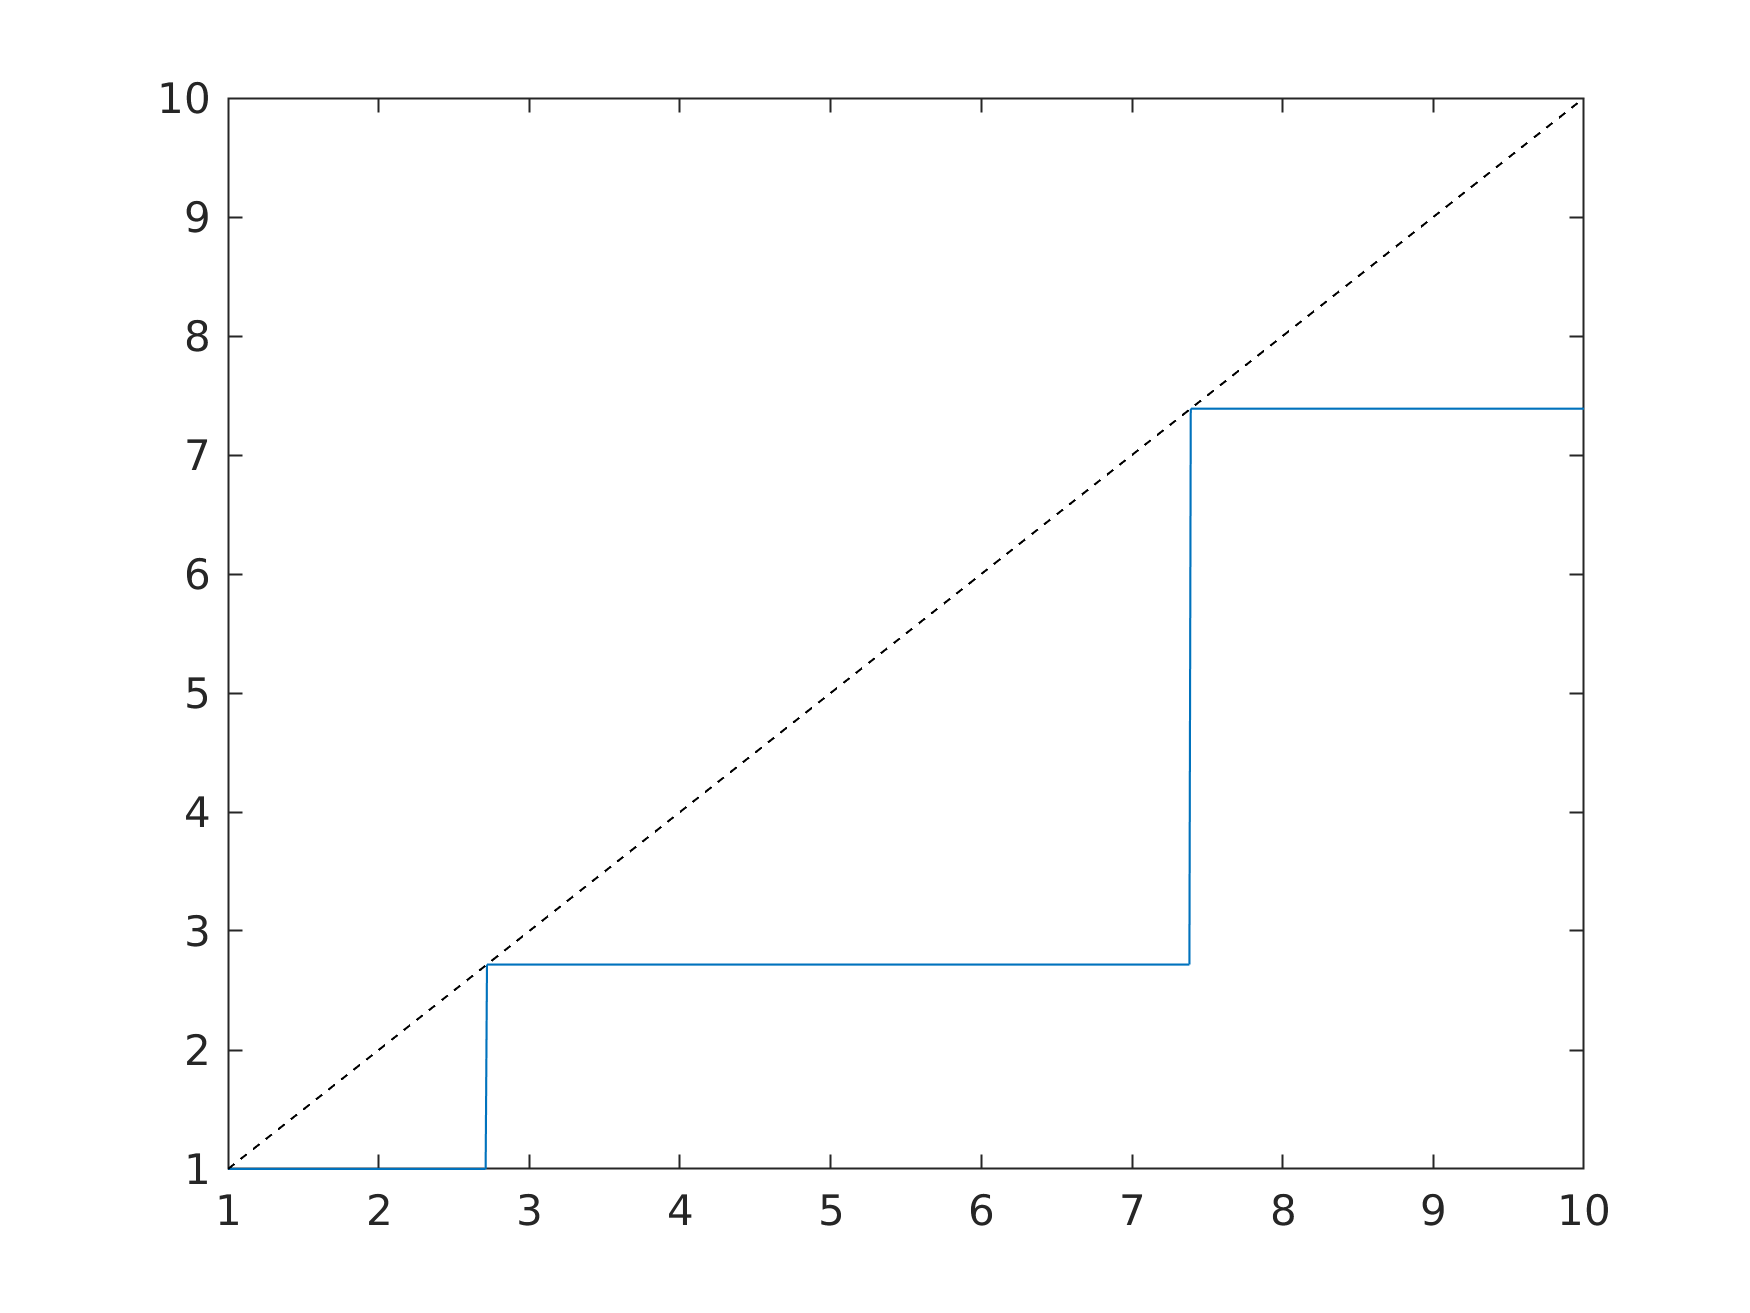
\includegraphics[width=0.6\textwidth]{plot.png}
\caption{Plot of vector x after 52 square roots and 52 square operations (blue) and the initial values of vector x (dashed)}
\end{figure}

After 52 repeated square roots, the value of a number (between 1 and 10) becomes very close to $1 \pm \epsilon$ with $\epsilon \ll 1$. To figure out what $\epsilon$ is we can rewrite $x^{2^{-n}}$ as $e^{2^{-n}\ln(x)}$. Now using a Taylor expansion we write the previous expression as:
\[
e^{2^{-n}\ln(x)} = 1 + 2^{-n} \ln(x) + \cancelto{\approx 0}{\frac{(2^{-n} \ln(x))^2}{2!}} + ...
\]
For large $n$ the higher order terms can be neglected. Now we write $\epsilon$ as:
\[
\epsilon = 2^{-n} \ln(x)
\]
When representing the number, $x^{2^{-n}}$, in a finite number of bits rounding error plays a large role when $n$ is large. As $n$ approaches $53$, $\epsilon$ reaches the order of machine epsilon, eps = $2^{-53}$, for double precision floating point numbers. This means that $\epsilon$ will be rounded to the nearest integer multiple of eps. When $x$ is a power of $e$, $x = e^{p}$, then $\epsilon = p \cdot 2^{-n}$. When $n = 52$ then $x^{2^{-n}}$ will be stored as $1 + p \cdot \mathrm{eps}$. Then after $n$ repeated squaring operations the floating point numbers (with rounding error) will resemble a staircase. Only starting values close to $e^p$ will be preserved.

\end{document}